% Manuel Lippert - Paul Schwanitz
% Physikalisches Praktikum

% Teilaufgabe 1

\section{Allgemeines zum Thema Chaos}
\label{sec:allgemeines}

\subsection{Dynamische Systeme}
\label{sub:dynamSys}
Ein \textit{\textbf{dynamisches System}} ist ein mathematisches Modell eines zeitabhängigen Prozesses, dessen Verlauf nur vom Anfangszustand abhängt. \citep{WikiDynSys}\\
Die Formulierung dieses Sachverhaltes in der Physik geschieht anhand von Differentialgleichungen mit dem Vektor $\vect{x}(t)=(x_1(t)$,...$x_n(t))\in\mathbb{R}^n$
\begin{gather}
    \dot{\vect{x}}(t)=\vect{F}(\vect{x}(t)),
    \label{eq:dynamDGL}
\end{gather}
dabei beschreibt $\vect{x}(t)$ den \textit{\textbf{Zustand}} des Systems zum Zeitpunkt $t\in\mathbb{R}$.\\
Das dynamische System ist vollständig determiniert, wenn ein Zustand $\vect{x}(t)$ angegeben ist. Aus diesem Zustand lassen sich alle vorangegangen und folgenden Zustände des Systems bestimmen. Dynamische Systeme können auch zeitdiskret angegeben werden, worauf aber hier nicht weiter eingegangen wird. \citep{Lueck}\\

\begin{itemize}
    \item[\textbf{1.}]\textbf{Phasenfluss}\\
    In der Mathematik wird ein dynamisches System durch den \textit{\textbf{Fluss}} bzw. \textit{\textbf{Phasenfluss}}  beschrieben. Unter dem \textit{Fluss} versteht man die Abbildung $\phi:\mathbb{R}^n\times\mathbb{R}\rightarrow\mathbb{R}^n$, welche die \textit{\textbf{Flussaxiome}} erfüllt \citep{Mat1}:
    \begin{gather}
        \begin{aligned}
            (1)~&\phi(\vect{x}_0,0)=\vect{x}_0\\
            (2)~&\phi(\phi(\vect{x}_0,t),s)=\phi(\vect{x}_0,t+s).
            \label{eq:flussaxiome}
        \end{aligned}
    \end{gather}
    Der \textit{Fluss} $\phi$ ordnet \textbf{jedem} Anfangszustand $\vect{x}_0$ einen neuen Zustand zum Zeitpunkt $t$ zu. \citep{Lueck}\\

    \item[\textbf{2.}]\textbf{Trajektorie}\\
    Der \textit{Fluss} $\phi$ kann mit dem \textit{Zustand} $\vect{x}(t)$ in Verbindung gebracht werden mit der Beziehung: $\vect{x}(t)=\phi_{\vect{x}_0}(t)=\phi(\vect{x}_0,t)$ mit festem $\vect{x}$, wobei nach  (\ref{eq:flussaxiome}) $\vect{x}(0)=\phi_{\vect{x}_0}(0)=\phi(\vect{x}_0,0)=\vect{x}_0$ gilt.\\
    Hierbei beschreibt $\phi_{\vect{x}_0}(t)$ die \textit{Lösungskurve}, welche auch \textit{Bahnkurve}, \textit{Orbit}, \textit{Phasenbahn} oder \textit{\textbf{Trajektorie}} des Flusses $\phi$ genannt wird und eine spezielle Lösung von (\ref{eq:dynamDGL}) darstellt, welche wiederum die Bewegung des Punktes $\vect{x}$ unter Wirkung des Flusses $\phi$ mit dem Anfangszustand $\vect{x}_0$ beschreibt. \citep{Lueck}\\
    Durch die Abhängigkeit der \textit{Trajektorien} vom Anfangszustand $\vect{x}_0$ kann gefolgert werden, dass sich \textit{Trajektorien} mit unterschiedlichen Anfangszuständen $\vect{x}_0$ nicht schneiden können. Es können aber unterschiedliche Anfangszustände $\vect{x}_0$ auf derselben \textit{Trajektorie} befinden und sich nur um eine Zeittranslation unterscheiden. \citep{Mat1}\\

    \item[\textbf{3.}]\textbf{Phasenraum}\\
    Der \textit{\textbf{Phasenraum}} oder \textit{\textbf{Zustandsraum}} beschreibt eine Menge aller Zustände oder eine Darstellung aller Trajektorien eines dynamischen Systems und bietet einen Überblick über das Verhalten der gesamten Differentialgleichung ohne diese explizit für $\vect{x}(t)$ lösen zu müssen. Der \textit{Phasenraum} ist hierbei eine Parameterdarstellung von der Differentialgleichung mit dem Zustand $\vect{x}(t)$ und dessen Ableitung $\dot{\vect{x}}(t)$ mit der Zeit $t$ als Parameter.\\ %!!! Quelle
    %Der \textit{Phasenraum} wird vom Zustand $\vect{x}(t)$ und dessen Ableitung $\dot{\vect{x}}(t)$ aufgespannt bzw. ist eine $(\vect{x}(t),\dot{\vect{x}}(t))$-Ebene, was eine Parameterdarstellung der Differentialgleichung über die Zeit $t$ darstellt.
    %In diesem \textit{Phasenraum} lässt sich dann ein Vektor $(\vect{x},\dot{\vect{x}})$ definieren, welcher auf die \textit{Trajektorien}, die sich mit dem Anfangszustand $\vect{x}_0$ änderen, zeigt. Die Ableitung dieses Vektors $\frac{\text{d}}{\text{d}t}(\vect{x},\dot{\vect{x}})=(\dot{\vect{x}},\ddot{\vect{x}})$ erzeugt ein \textit{Vektorfeld} bzw. ein \textit{Richtungsfeld} der Differentialgleichung, dessen Vektoren tangential auf den \textit{Trajektorien} steht.

    \item[\textbf{4.}]\textbf{Attraktor}\\
    In (\ref{eq:dynamDGL}) wird ein Vektorfeld $\vect{F}$ im Phasenraum definiert, welches als Geschwindigkeitfeld des Phasenflusses $\phi$ angesehen werden kann.\\ Durch Betrachtung der Divergenz des Vektorfelds $\nabla\vect{F}$ kann eine Aussage getroffen werden über die Rate mit dem sich ein Volumenelement $V$ unter der Wirkung des Flusses verändert. Zwei Fälle sind hier besonders hervorzuheben:
    \begin{gather}
        \begin{aligned}
            (1)~&\nabla\cdot\vect{F}=0\Rightarrow \dot{V}=0 \Rightarrow~\text{Konservatives System}\\
            (2)~&\nabla\cdot\vect{F}<0\Rightarrow \dot{V}<0 \Rightarrow~\text{Dissipatives System}
        \end{aligned}
    \end{gather}
    In einem dissipativen System laufen die Trajektorien nach einer Einlaufsphase (transiente Bewegung) in einem begrenzten Bereich im Phasenraum, welchen man als \textit{\textbf{Attraktor}} bezeichnet (Bewegung auf \textit{Attraktor}: permante oder posttransiente Bewegung). Ein Attraktor weist folgende Eigenschaften auf:
    \begin{itemize}
        \item[(1)] Kompakte Menge im Phasenraum
        \item[(2)] Invariant unter der Wirkung des Flusses
        \item[(3)] Volumen des Attraktors ist Null
        \item[(4)] Eine beliebige Obermenge des Attraktors schrumpft unter der Wirkung des Flusses auf den Attraktor selbst zusammen   
    \end{itemize}
    \textbf{Arten von Attraktor}
    \begin{center}
        \begin{tabular}{ccc}
            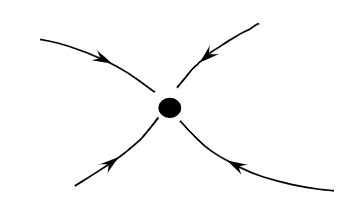
\includegraphics[width=4cm]{FixpunktAttraktor.png}
            & 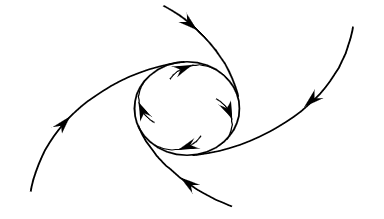
\includegraphics[width=4cm]{GrenzzyklusAttraktor.png}
            & 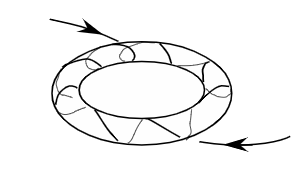
\includegraphics[width=4cm]{TorusAttraktor.png}
        \end{tabular}
        \captionof{figure}{Fixpunkt, Grenzzyklus, Tours- bzw. Ringattraktor}
        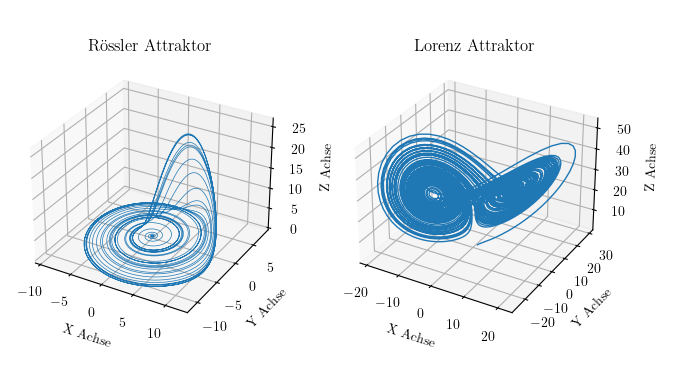
\includegraphics[width=14cm]{SeltsameAttraktoren.png}
        \captionof{figure}{Seltsame Attraktoren}
    \end{center}
\end{itemize}

\subsection{Deterministisches Chaos}
\label{sub:determChaos}
% TODO: #17 FzV 2.1.3 @PaulSchwanitz

\subsection{Fouriertransformation und Leistungsspektrum}
\label{sub:fouriertrafo}
% TODO: #19 FzV 2.1.4 @PaulSchwanitz

\subsection{Darstellungsweisen eines chaotischen Attraktor}
\label{sub:darstellungAttraktor}
% TODO: #20 FzV 2.1.5 @ManeLippert